\documentclass[12pt]{article}
\usepackage{amsfonts}
\usepackage{amsmath}
\usepackage{bm}
\usepackage{bbm}
\usepackage{graphicx}
\usepackage{geometry}[margin=1in]
\usepackage{subcaption}
\usepackage{array}
\usepackage{multirow}
\usepackage{hyperref}

% for algorithms
\usepackage[linesnumbered,ruled]{algorithm2e}

\usepackage{natbib}
\usepackage{multicol}
\bibliographystyle{plainnat}
% set path for bibliography

\title{Regionally Additive Models: Explainable-by-design models minimizing feature interactions}

\newcommand{\dfdx}{\frac{\partial f}{\partial x_s}}
\newcommand{\Rd}{\mathbb{R}^d}
\newcommand{\xb}{\mathbf{x}}
\newcommand{\xc}{\mathbf{x_c}}
\newcommand{\xcc}{\mathbf{x_{/s}}}
\newcommand{\fxc}{f^{(\xc)}}
\newcommand{\fxs}{f^{(x_s)}}
\newcommand{\Xcal}{\mathcal{X}}
\newcommand{\Ycal}{\mathcal{Y}}
\newcommand{\when}[1]{\mathbbm{1}_{#1}}

\author{Vasilis Gkolemis}


\begin{document}
\maketitle

\begin{abstract}
Generalized Additive Models (GAMs) are widely utilized explainable-by-design models in various applications.
However, their assumption of independence among features can lead to suboptimal performance when violated.
To overcome this limitation, we introduce Regionally Additive Models (RAMs), a novel class of explainable-by-design models.
RAMs mitigate the issue by identifying subregions in the feature space where interactions are minimized and fitting multiple GAMs accordingly.
The RAM framework consists of three steps.
Firstly, we train a black-box model.
Secondly, using Regional Effect Plots, we identify subregions where the black-box model exhibits near-local additivity.
In these subregions, the effect of each feature on the target is independent of the values of other features.
Lastly, we fit a GAM specifically for each identified subregion.
We validate the effectiveness of RAMs through experiments on both a synthetic example and real-world datasets.
The results confirm that RAMs offer improved expressiveness compared to GAMs while maintaining interpretability.
\end{abstract}

\section{Introduction}


% Paragraph for Motivating about Regionally Additive Models
Generalized Additive Models (GAMs)~\citep{hastie1987generalized} are a popular class of explainable by design (x-by-design) models.
Their popularity stems from their seamless interpretability; since they are a linear (additive) combination of univariate functions,
\(f(\xb) = c + \sum_{s=1}^D f_s(x_s)\), each individual univariate function (component) can be readily visualized and comprehended in isolation.
However, GAM's main limitation is that they cannot express interactions between features.
To mitigation this limitation, some approaches~\citep{lou2013accurate} extend them enabling pairwise interactions,
i.e., \(f(\xb) = c + \sum_{s=1}^D f_s(x_s) + \sum_{s=1}^D \sum_{c \neq s} f_{sc}(x_s, x_c)\).
Pairwise interactions can also be visualized and understood in isolation, so these models also maintain their x-by-design nature.
Unfortunately, this does not hold for any interaction that involves more than two features, thus, the expressiveness of GAMs is limited to capturing up to two-feature interactions.

% Paragraph for Motivating about Regionally Additive Models
To overcome this limitation, we propose Regionally Additive Models (RAMs), a novel class of x-by-design models,
that fits multiple GAMs to subregions of the feature space where interactions are minimized.
Our approach consists of a three-step pipeline.
First, we fit a black-box model to capture all high-order interactions.
Second, we identify the subregions where the black-box model is nearly locally additive.
Finally, we train a GAM specifically for each identified subregion.

\section{Background and motivation}
\label{sec:motivation}

Consider the black-box function \(f(\xb) = 8x_2\when{x_1 > 0}\when{x_3=0}\)
with \(x_1, x_2 \sim \mathcal{U}(-1,1)\) and \(x_3 \sim Bernoulli(0,1)\).
Although very simple, a GAM would fail to learn this mapping due to
the existence of the three-features interaction term $8x_2\when{x_1 > 0}\when{x_3=0}$.
As we see in Figure~\ref{subfig:global_gam}, a GAM misleadingly learns that $\hat{f}(\xb) \approx 2x_2$,
because in $\frac{1}{4}$ of the cases ($x_1 > 0 \text{ and } x_3 = 0$) the impact of $x_2$ to the output is $8x_2$,
and in the rest $\frac{3}{4}$ of the cases the impact of $x_2$ to the output is $0$.
However, if splitting the input space in two subregions we observe that \(f\) is additive in each one (regionally additive):
%
\begin{equation}
    \label{eq:regionally_additive}
    f(\xb) = \begin{cases} 8x_2 & \text{if } x_1 > 0 \text{ and } x_3 = 1 \\ 0 & \text{otherwise} \end{cases}
\end{equation}
%
Therefore, if we knew the appropriate subregions,
namely, \(\mathcal{R}_{21} = \{x_1 > 0 \text{ and } x_3 = 0\}\)
and  \(\mathcal{R}_{22} = \{x_1 \leq 0 \text{ or } x_3 = 1\}\),
we could split the impact of $x_2$ appropriately and fit the following model to the data:

\begin{equation}
    \label{eq:regional_gam}
    f^{\mathtt{RAM}}(\xb) = f_1(x_1) + f_{21}(x_2) \when{(x_1, x_3) \in \mathcal{R}_{21}} + f_{22}(x_2) \when{(x_1, x_3) \in \mathcal{R}_{22}} + f_3(x_3)
\end{equation}
%
Equation~\eqref{eq:regional_gam} represents a Regionally Additive Model (RAM), which is simply a GAM fitted on each subregion of the feature space.
Importantly, RAM's enhanced expressiveness does not come at the expense of interpretability.
As we observe in Figures~\ref{subfig:regional_gam_1} and~\ref{subfig:regional_gam_2}, we can still visualize and comprehend each univariate function in isolation, exactly as we would do with a GAM,
with the only difference being that we have to consider the subregions where each univariate function is active,
The key challenge of RAMs is to appropriately identify the subregions where the black-box function is (close to) regionally additive.
For this purpose, as we will see in Section~\ref{subsec:regional_effect_methods}, we propose a novel algorithm that is based on the idea of
regional effect plots.

\begin{figure}[htbp]
    \centering
    \begin{subfigure}{0.32\textwidth}
        \centering
        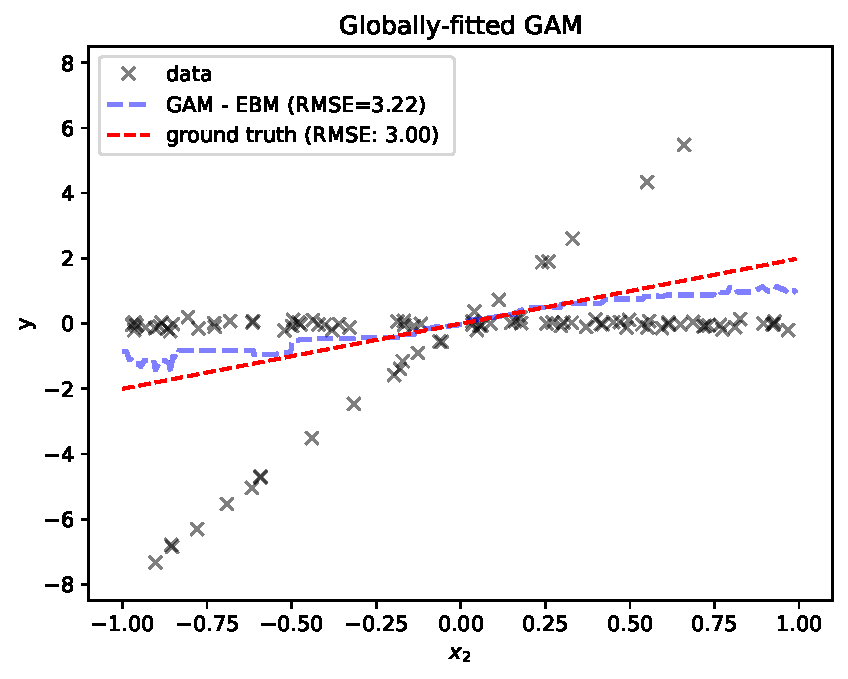
\includegraphics[width=\textwidth]{figures/global_GAM}
        \caption{\(f_2(x_2)\)}
        \label{subfig:global_gam}
    \end{subfigure}
    \begin{subfigure}{0.32\textwidth}
        \centering
        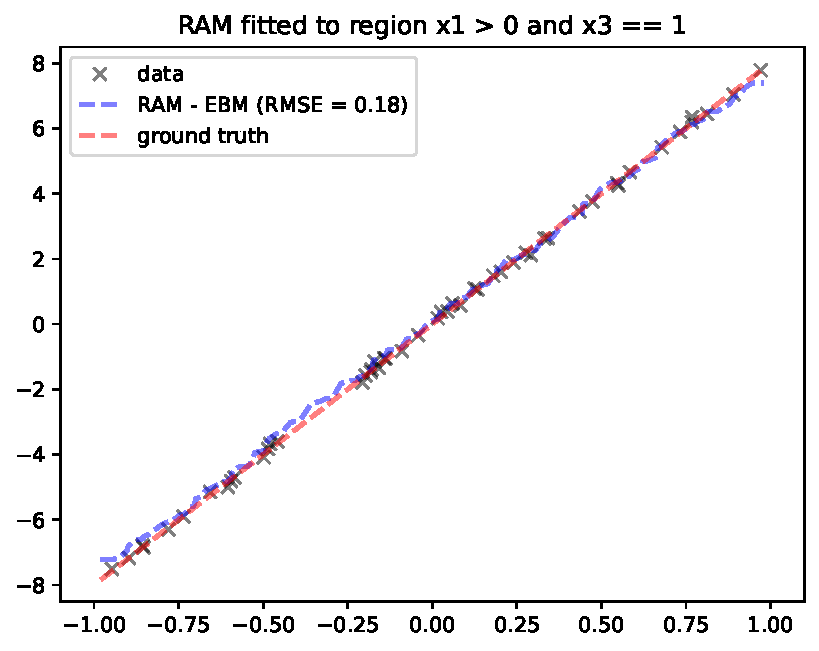
\includegraphics[width=\textwidth]{figures/regional_gam_subreg_1}
        \caption{\(f_2(x_2) \when{x_1 > 0 \text{ and } x_3 = 1}\)}
        \label{subfig:regional_gam_1}
    \end{subfigure}
    \begin{subfigure}{0.32\textwidth}
        \centering
        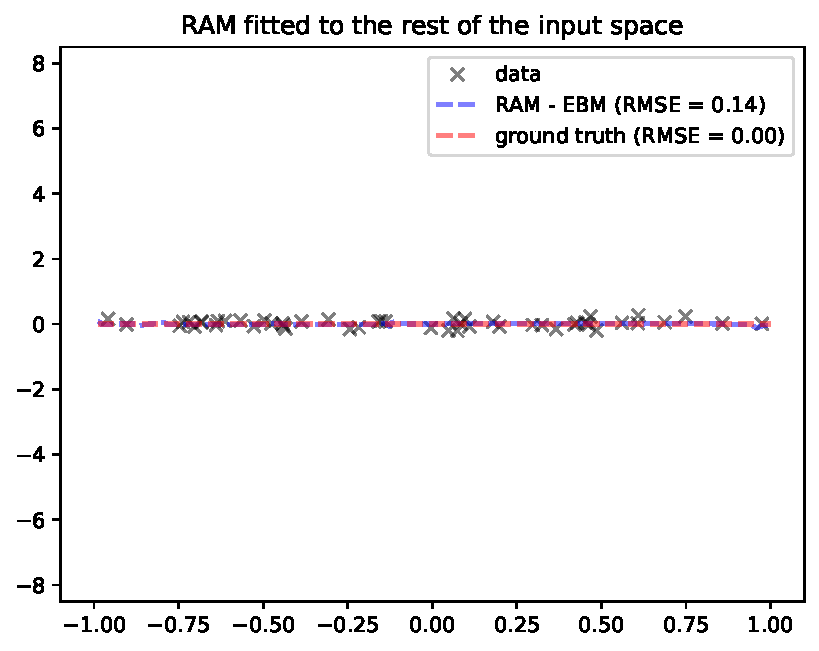
\includegraphics[width=\textwidth]{figures/regional_gam_subreg_2}
        \caption{\(f_2(x_2) \when{x_1 \leq 0 \text{ or } x_3 \neq 1}\)}
        \label{subfig:regional_gam_2}
    \end{subfigure}
    \caption{Caption for the entire figure}
    \label{fig:ram_example}
\end{figure}


\section{The RAM framework}

The RAM framework consists of a three-step pipeline; (a) fit a black-box model (Section~\ref{subsec:fit_black_box}),
(b) identify subregions with minimal interactions (Section~\ref{subsec:regional_effect_methods}) and
(c) fit a GAM to each subregion (Section~\ref{subsec:fitting_gams}).
Throughout this section, we will use the following notation.
Let \(\Xcal \in \Rd\) be the \(d\)-dimensional feature space, \(\Ycal\) the target space and \(f(\cdot) : \Xcal \rightarrow \Ycal\) the black-box function.
We use index \(s \in \{1, \ldots, d\}\) for the feature of interest and \(/s = \{1, \ldots, D\} - s\) for the rest.
For convenience, we use \((x_s, \xcc)\) to refer to \((x_1, \cdots , x_s, \cdots, x_D)\) and, equivalently, \((X_s, X_{/s})\) instead of \((X_1, \cdots , X_s, \cdots, X_D)\) when we refer to random variables.
The training set \(\mathcal{D} = \{(\xb^i, y^i)\}_{i=1}^N\) is sampled
i.i.d.\ from the distribution \(\mathbb{P}_{X,Y}\).
%Finally, \(f^{\mathtt{<method>}}(x_s)\) denotes how \(\mathtt{<method>}\)
%defines the feature effect and \(\hat{f}^{\mathtt{<method>}}(x_s)\)
%how it estimates it from the training set.

\subsection{First step: Fit a black-box function}
\label{subsec:fit_black_box}

In the initial step of the pipeline, we fit a black-box function \(f(\cdot)\) to the training set
\(\mathcal{D} = \{(\xb^i, y^i)\}_{i=1}^N\) to accurately learn the underlying mapping \(f(\cdot) : \Xcal \rightarrow \Ycal\).
While any black-box function can theoretically be employed in this stage,
for utilizing the DALE approximation, as we will show in the next step,
it is necessary to select a differentiable function.
Recent advancements have demonstrated that differentiable Deep Learning models,
specifically designed for tabular data~\citep{arik2021tabnet}, are capable of achieving state-of-the-art performance,
making them a suitable choice for this step.


\subsection{Second step: Find subregions}
\label{subsec:regional_effect_methods}

In this step, we use regional effect methods~\citep{herbinger2023decomposing, herbinger2022repid}
to identify the regions where the black-box function is (close to) regionally additive.
% Describe the goal of the regional effect methods
Regional effect methods yield for each individual feature \(s\), a set of \(T_s\) non-overlapping regions,
denoted as \(\{\mathcal{R}_{st}\}_{t=1}^{T_s}\) where \(\mathcal{R}_{st} \subseteq \Xcal_{/s}\).
Note that, the number of non-overlapping regions can be different for each feature ($T_s$),
the regions \(\{\mathcal{R}_{st}\}_{t=1}^{T_s}\) are disjoint
and their union covers the entire feature space \(\Xcal_{/s}\).
The primary objective is to identify regions in which the impact of the \(s\)-th feature on the output is
\textit{relatively independent} of the values of the other features \(\xcc\).
To better grasp this objective, if we decompose the impact of the \(s\)-th feature on the output $y$ into two terms:
\(f_s(x_s, \xcc) = f_{s,ind}(x_s) + f_{s, int}(x_s, \xcc)\),
where \(f_{s,ind}(\cdot)\) represents the independent effect
and \(f_{s, int}(\cdot)\) represents the interaction effect,
the objective is to identify regions \(\{\mathcal{R}_{st}\}_{t=1}^{T_s}\) such that the interaction effect is minimized.
Regionally Additive Models (RAM) formulate the mapping \(\mathcal{X} \rightarrow \mathcal{Y}\) as:

\begin{equation}
\label{eq:ram_formulation}
f^{\mathtt{RAM}}(\xb) = c + \sum_{s=1}^D \sum_{t=1}^{T_s} f_{st}(x_s) \when{\xcc \in \mathcal{R}_{st}}, \quad \xb \in \Xcal
\end{equation}
%
In the above formulation, \(f_{st}(\cdot)\) is the component of the \(s\)-th feature which is active on the \(t\)-th region.
RAM can be viewed as a GAM with \(T_s\) components per feature where each component is applied to a specific region \(\mathcal{R}_{st}\).
To facilitate this interpretation, we can define an enhanced feature space \(\Xcal^\mathtt{RAM}\) defined as:

\begin{equation}
\label{eq:ram_feature_space}
\begin{aligned}
\Xcal^{\mathtt{RAM}} &= \{x_{st} | s \in \{1, \ldots, D\}, t \in \{1, \ldots, T_s\}\} \\
x_{sk} &= \begin{cases}
x_s, & \text{if } \xcc \in \mathcal{R}_{sk} \\
0, & \text{otherwise}
\end{cases}
\end{aligned}
\end{equation}
%
and then define RAM as a typical GAM on the extended feature space \(\Xcal^{\mathtt{RAM}}\):

\begin{equation}
\label{eq:ram_formulation2}
f^{\mathtt{RAM}}(\xb) = c + \sum_{s,t} f_{st}(x_{st}) \quad \xb \in \Xcal^{\mathtt{RAM}}
\end{equation}
%
Equations~\ref{eq:ram_formulation} and~\ref{eq:ram_formulation2} are equivalent.
To gain a better understanding of the latter formulation, consider the toy example described in Section~\ref{sec:motivation}.
To minimize the impact of feature interactions, we need to divide feature \(x_2\) into two subregions,
\(\mathcal{R}_{21} = \{x_1 > 0 \text{ and } x_3 = 1\}\) and \(\mathcal{R}_{22} = \{x_1 \leq 0 \text{ or } x_3 = 0\}\).
This division results in an augmented feature space \(\Xcal^{\mathtt{RAM}} = (x_1, x_{21}, x_{22}, x_3)\)
and a RAM formulation of the form: \(f^{\mathtt{RAM}}(\xb) = f_1(x_1) + f_{21}(x_{21}) + f_{22}(x_{22}) + f_3(x_3)\).


\subsubsection{Proposed Approach}

To identify the regions of the input space where the impact of feature interactions is reduced,
we have developed a regional effect method influenced by the research conducted by
\citet{herbinger2023decomposing} and \citet{gkolemis2023dale}.
\citet{herbinger2023decomposing} introduced a versatile framework for detecting such regions,
where one of the proposed methods is the Accumulated Local Effects~\citep{apley2020visualizing}.
We have adopted their approach with two notable modifications.
First, instead of using the ALE plot, we employ the Differential ALE (DALE) method introduced by \citet{gkolemis2023dale},
which provides considerable computational advantages when the underlying black-box function is differentiable.
Second, we utilize variable-size bins, instead of the fixed-size ones in DALE, because the result in a more accurate approximation.

\paragraph{DALE formulation}

DALE gets as input the black-box function \(f(\cdot)\)
and the dataset \(\mathcal{D} = \{(\xb^i, y^i)\}_{i=1}^N\),
and returns the effect (impact) of a specific feature $s$ on the output $y$:
%
\begin{equation}  \label{eq:DALE_accumulated_mean_est}
  \hat{f}^{\mathtt{DALE}}(x_s) = \Delta x \sum_{k=1}^{k_x} \underbrace{\frac{1}{|\mathcal{S}_k|} \sum_{i:\mathbf{x}^{(i)} \in
    \mathcal{S}_k} \dfdx(\mathbf{x}^i)}_{\hat{\mu}(z_{k-1}, z_k)})
\end{equation}
%
For more details on the DALE method, please refer to the original paper~\citep{gkolemis2023dale}.
In the above equation, \(k_x\) is the index of the bin such that
\(z_{k_x-1} \leq x_s < z_{k_x} \) and \(\mathcal{S}_k\)
is the set of the instances of the \(k\)-th bin, i.e.
\( \mathcal{S}_k = \{ \xb^i : z_{k-1} \leq x^{(i)}_s < z_{k} \} \).
In short, DALE computes the average effect (impact) of the feature \(x_s\) on the output,
by, first, dividing the feature space into $K$ equally-sized bins, i.e., \(z_0, \ldots, z_K\)
second, computing the average effect in each bin \(\hat{\mu}(z_{k-1}, z_k)\) (bin-effect) as the average of the instance-level effects inside the bin,
and, finally, aggregating the bin-level effects.

\paragraph{DALE for feature interactions}

In cases where there are strong interactions between the features,
the instance-level effects inside each bin deviate from the average bin-effect.
We can measure such deviation using the standard deviation of the instance-level effects inside each bin (bin-deviation):

\begin{equation}
  \label{eq:var_bin_approx}
  \hat{\sigma}^2(z_{k-1}, z_k) = \frac{1}{|\mathcal{S}_k| - 1}
\sum_{i:\mathbf{x}^i \in \mathcal{S}_k} \left ( \dfdx(\mathbf{x}^i) -
  \hat{\mu}(z_{k-1}, z_k) \right )^2
\end{equation}
%
and the interaction between the feature \(x_s\) and the rest of the features along the whole \(s\)-th dimension
with the aggregated bin-deviation:
\begin{equation}
  \label{eq:DALE_interaction}
  \mathcal{H}_s = \sqrt{ \sum_{k=1}^{k_x} (z_k - z_{k-1})^2 \hat{\sigma}^2(z_{k-1}, z_k) }
\end{equation}
%
Eq.~\eqref{eq:DALE_interaction} measures the interaction between the feature \(x_s\) and the rest of the features.
It takes values in the range \([0, \infty)\) with zero indicating that \(x_s\) does not interact with the rest of the features,
i.e., the underlying black box function can be written as $f(\xb) = f_s(x_s) + f_{/s}(x_{/s})$.
In all other cases, $\mathcal{H}_s$ is greater than zero and the higher the value, the stronger the interaction.

A final detail, is that in order to have a more robust estimation of the bin-effect and the bin-deviation,
we use variable-size bins instead of the fixed-size ones in DALE.
In particular, we start with a dense fixed-size grid of bins and we iteratively merge the neighboring bins with similar
bin-effect and bin-deviation until all bins have at least $n_{\min}$ instances.
In this way, we can have a more accurate approximation of the bin-effect and the bin-deviation.

\paragraph{Subregions as an optimization problem}

In the same way that we can estimate the feature effect and the feature interactions for the $s$-th feature in the whole input space,
using Eq.~\eqref{eq:DALE_accumulated_mean_est} and Eq.~\eqref{eq:DALE_interaction},
we can also estimate the effect and the interactions in a subregion of the input space \(\mathcal{R}_{st} \subset \mathcal{X}\).
We denote the equivalent regional qunatities as $f^{\mathtt{DALE}}_{\mathcal{R}_{st}}(x_s)$ and $\mathcal{H}_{\mathcal{R}_{st}}$.
$f^{\mathtt{DALE}}_{\mathcal{R}_{st}}(x_s)$ and $\mathcal{H}_{\mathcal{R}_{st}}$ are defined exactly as in
Eq.~\eqref{eq:DALE_accumulated_mean_est} and Eq.~\eqref{eq:DALE_interaction} respectively,
with the only difference that instead of using the whole dataset \(\mathcal{D}\) to compute the regional bin-effect $\hat{\mu}_{\mathcal{R}_{st}}(z_{k-1}, z_k)$
and the regional bin-deviation $\hat{\sigma}_{\mathcal{R}_{st}}^2(z_{k-1}, z_k)$,
we use only the instances that belong to the subregion \(\mathcal{R}_{st}\), i.e. $\xb^i: x_s^i \in \mathcal{S}_k \land x_{s}^i \in \mathcal{R}_{st}$.
Therefore, in order to minimize the interactions of a particular feature $s$ we search for a set of regions \(\{\mathcal{R}_{st}\}_{t=1}^{T_s}\),
that minimize:

\begin{equation}
  \label{eq:optimal_subregions}
  \begin{aligned}
    & \underset{\{\mathcal{R}_{st}\}_{t=1}^{T_s}}{\text{minimize}}
    & & \mathcal{L} = \sum_{t=1}^{T_s} \mathcal{H}_{\mathcal{R}_{st}} \\
    & \text{subject to}
    & & \bigcup_{t=1}^{T} \mathcal{R}_{st} = \mathcal{X} \\
    & & & \mathcal{R}_{st} \cap \mathcal{R}_{s\tau} = \emptyset, \quad \forall t \neq \tau
  \end{aligned}
\end{equation}
%



\paragraph{Proposed solution}

For minimizing Eq.~\eqref{eq:SE}, we develop a tree-based algorithm, similar to the one proposed by~\citep{herbinger2023decomposing}.
The backbone of the algorithm is described in Algorithm~\ref{alg:subregion_detection}.
For each feature $s$, we search for the $T$ optimal splits.
To better understand the algorithm, let's take the toy example of Section~\ref{sec:motivation}.
The subregions are searched independently for each feature $s \in \{1, \ldots, D\}$.
For feture $s=2$, we start by searching for the optimal split for the first level of the tree.
The candidate features for defining the first level split are $x_1$ and $x_3$.
The algorithm~\ref{alg:single_feature_subregion} is responsible to find the optimal first level split.
First, it defines the candidate split points for each feature.
Since $x_1$ is a continuous feature, the candidate split points are a linearly spaced grid of $p$ points in the range $[-1, 1]$,
where $P$ is a hyperparameter of the algorithm, set to 10 in the experiments.
Therefore, the candidate split points are $p = \{-1, -0.8, -0.6, \ldots, 0.8, 1\}$ and
the corrsponding subregions are $\mathcal{R}_{21} = \{ \mathbb{R}^2 : x_1 \leq p \}$ and $\mathcal{R}_{22} = \{ \mathbb{R}^2 : x_1 > p \}$.
Since $x_3$ is categorical, the candidate split points are the unique values of $x_3$, i.e. $\{0, 1\}$
and the corresponding subregions are $\mathcal{R}_{21} = \{ \mathbb{R}^2 : x_3 = 0 \}$ and $\mathcal{R}_{22} = \{ \mathbb{R}^2 : x_3 = 1 \}$.
For each candidate split point, the algorithm computes the corresponding subregions and the corresponding $\mathcal{H}_{\mathcal{R}_{st}}$.
and selects the split point that minimizes the weighted level of interactions, as defined by Algorithm~\ref{alg:get_interaction}.
Suppose that the optimal first-level subregions are $\mathcal{R}_{21} = \{ \mathbb{R}^2 : x_3 = 0 \}$ and $\mathcal{R}_{22} = \{ \mathbb{R}^2 : x_3 \neq 0 \}$.
The algorithm then proceeds to the second level of the tree.
For the second level, the first split is fixed, i.e. the are two datasets split according to the first-level split and the algorithm searches for the optimal second-level split.
The candidate features for defining the second level split are $x_3$.

The output of algorithm~\ref{alg:subregion_detection} is a set of $T$ splits per feature $s$.
It is imporant to note, that since not all splits lead to an important decrease in the level of interactions,
we post-process the splits by pruning all splits that do not decrease the loss function by more than a threshold $\epsilon$.
The final set of splits is denoted as $\{\mathcal{R}_{st}\}_{t=1}^{T_s}$.


\begin{algorithm}
\caption{Regionally Additive Model (RAM) training}
\label{alg:ram}
\SetAlgoLined
\SetKwInOut{Input}{Input}
\SetKwInOut{Output}{Output}
\BlankLine
\Input{A dataset $(X, y)$}
\Output{A trained RAM model $f^{\mathtt{RAM}}$}
  \BlankLine
  Train a differentiable black box model $f$ using $(X, y)$\;
  \tcc{Detect subregions for all features}
  $\left\{\mathcal{R}_{st}|s\in\left\{1,\ldots,D\right\}, t\in\left\{1,\ldots,T_s\right\}\right\}$ = DetectSubregions($X$, $y$, $f$)\;
  Create the extended feature space $\mathcal{X}^{\mathtt{RAM}}$ using all
  $\mathcal{R}_{st}$, as in Eq. \eqref{eq:ram_feature_space} \;
  Fit a GAM in $\mathcal{X}^{\mathtt{RAM}}$ \tcp*{i.e., train each $f_{st}$ using
    only data in $\mathcal{R}_{st}$}
  \Return{$f^{\mathtt{RAM}}(\xb) = c + \sum_{s,t} f_{st}(x_{st}), \quad \xb \in \Xcal^{\mathtt{RAM}}$}
\end{algorithm}

\begin{algorithm}
\caption{Detection of Subregions using DALE}
\label{alg:subregion_detection}
\SetAlgoLined
\SetKwInOut{Input}{Input}
\SetKwInOut{Output}{Output}
\BlankLine
\Input{Data matrix $X$, Black box model $f$, Maximum Depth $T$}
\BlankLine
\Output{Subregions $\mathcal{R}_{sK}$ for all features $s$ and depth $K=2^T$}
\BlankLine
Initialize empty arrays for \texttt{loss}, \texttt{position}, and \texttt{feature\_c}
\BlankLine
\For{$s = 1$ to $D$}{
X\_list, J\_list = [X], [J] \tcp*{Init lists}
\For{$t = 1$ to $T$}{
    \tcc{Find best split}
    L, p, c, X\_list, J\_list $\gets$ BestSplit(X\_list, J\_list, s, is\_cat)\;
    \tcc{Store best split}
    loss[s, t], position[s, t], feature\_c[s, t] $\gets$ L, p, c
}
}
\Return{loss, position, feature\_c}
\end{algorithm}

\begin{algorithm}
\caption{BestSplit}
\label{alg:single_feature_subregion}
\SetAlgoLined
\SetKwInOut{Input}{Input}
\SetKwInOut{Output}{Output}

\Input{X\_list, J\_list, s, c, is\_cat}
\Output{BestSplits}

% Initialize variables
\BlankLine
L[c, p] $\gets$ None\; % \Comment{List to store interaction values}
\For{c $s = 1$ to $D$ \textnormal{if} c $\neq$ s}{
    is\_cat $\gets$ IsCategorical(X\_list, c)\;
    positions $\gets$ GetPositions(X\_list, c, is\_cat)\;
    L\_pos $\gets$ []\; % \Comment{List to store interaction values}
    \For{p \textnormal{in} positions}{
        X\_split, J\_split $\gets$ SplitDataset(X\_list, J\_list, c, p, is\_cat)\;
        L $\gets$ GetInteraction(X\_split, J\_split)\;
    }
}
L\_min $\gets$ min(L)\;
c\_min, p\_min = argmin(L)\;
is\_cat $\gets$ IsCategorical(X\_list, c\_min)\;
X\_split, J\_split $\gets$ SplitDataset(X\_list, J\_list, c\_min, p\_min, is\_cat)\;

\Return{L\_min, p\_min c\_min, X\_split, J\_split}
\BlankLine
\end{algorithm}

\begin{algorithm}
\caption{GetInteraction}
\label{alg:get_interaction}
\SetAlgoLined
\SetKwInOut{Input}{Input}
\SetKwInOut{Output}{Output}
\Input{$X\_list$, $J\_list$, $min\_points$}
\Output{weighted average of interaction levels}
N $\gets$ total number of items in $X\_list$\;
W $\gets$ []\;
L $\gets$ []\;
\For{$i$ in len($X\_list$)}{
    X $\gets$ X\_list[i]\;
    J $\gets$ J\_list[i]\;
    \uIf{$|X|$ < min\_points}{
      Append $\infty$ to L\;
    }
    \Else{
        Append $\mathcal{L}(X, J)$ to $L$\;
    }
    Append $\frac{|X|}{N}$ to $W$\;
}
\Return $\text{sum}(L \cdot W)$\;
\end{algorithm}



\paragraph{Computational Complexity}

Algorithm~\ref{alg:subregion_detection} has a computational complexity of $\mathcal{O}(D \cdot T)$.
and Algorithm~\ref{alg:single_feature_subregion} has a computational complexity of $\mathcal{O}(D-1 \cdot P \cdot N)$
where $D$ is the number of feature, $N$ is the number of samples, $T$ is the maximum depth of the tree and $P$ is the number of query postitions.
The computational complexity of the proposed method is therefore $\mathcal{O}(D \cdot (D-1) \cdot T \cdot P \cdot N)$.
However, in practice, the number of query positions $P$ and the maximum depth $T$ are small numbers.
Therefore, the computational complexity of the proposed method is $\mathcal{O}(D^2 \cdot N)$.

\subsection{Fitting the GAMs}
\label{subsec:fitting_gams}

\subsubsection{Objective}

\subsubsection{Proposed Approach}

\subsection{Discussion}

Recently, a number of methods have been proposed to extend traditional GAMs and make them more expressive.
The majority of the ideas follow one of the following research directions;
The first one targets on representing the main components of a GAM $\{ f_i(x_i) \}$ with novel models.
For example, \citet{agarwal2021neural} who used an end-to-end neural network for learning the main components.
The second one focuses on extending the GAMs to model interactions between the features.
For example, \citet{lou2013accurate} proposed Explainable Boosting Machines (EBMs) which are a generalized additive model with pairwise interaction terms.
It is worth noting that the proposed method is orthogonal to the aforementioned research directions.
As we will show in the experiments, the proposed method can be used in conjunction with any of the
aforementioned methods to improve the accuracy of the resulting model, while maintaining the interpretability of the model.

\section{Experiments}

\begin{table}[htbp]
  \centering
  \caption{Result Comparison}
  \label{tab:sample}
  \begin{tabular}{l|c|cccc}
      \hline
      & \textbf{Black-box} & \multicolumn{4}{c}{\textbf{x-by-design}} \\
      \hline
      \hline
      & all orders & \multicolumn{2}{c}{1\textsuperscript{st} order} & \multicolumn{2}{c}{2\textsuperscript{nd} order} \\
      \hline
      \hline
      & \textbf{DNN} & \textbf{GAM} & \textbf{RAM} & \textbf{GAM}$^2$ & \textbf{RAM}$^2$ \\
      \hline
      Bike Sharing      & 0.254 & 0.549 & 0.430 & 0.298 & 0.278 \\
      \hline
      California Housing      & 0.369 & 0.600 & 0.535 & 0.554 & 0.514 \\
  \end{tabular}
\end{table}

We evaluate the proposed approach on two typical tabular datasets, namely the Bike-Sharing Dataset~\citep{misc_bike_sharing_dataset_275}
and the California Housing Dataset~\citep{pace1997sparse}.

\paragraph{Bike-Sharing Dataset}

The Bike-Sharing dataset contains the hourly bike rentals in the state of Washington DC over the period 2011 and 2012.
The dataset contains a total of 14 features, out of which 11 are selected as relevant for the purpose of prediction.
The majority of these features involve measurements related to environmental conditions,
such as $X_{\mathtt{month}}$, $X_{\mathtt{hour}}$, $X_{\mathtt{temperature}}$, $X_{\mathtt{humidity}}$ and $X_{\mathtt{windspeed}}$.
Additionally, certain features provide information about the type of day, for example, whether it is a working day ($X_{\mathtt{workingday}}$) or not.
The target value \( Y_{\mathtt{count}}\) is the bike rentals per hour, which has mean value
\(\mu_{\mathtt{count}} = 189\) and standard deviation \(\sigma_{\mathtt{count}} = 181\).

% Training - Evaluation - Region Extraction
As a black-box model, we train for \(60\) epochs a fully-connected Neural Network with 6 hidden layers, using the Adam optimizer with a learning rate of $0.001$.
The model attains a root mean squared error of \( 0.25 \cdot 181 \approx 45\) counts on the test set.
Subsequently, we extract the subregions, searching for splits up to a maximum spliting depth of \(T=3\).
Following the postprocessing step, we find that the only split that substantially reduces the level of interactions within the subregions is based on the feature
$X_{\mathtt{hour}}$. This feature is divided into two subgroups: $X_{\mathtt{hour}} | \when{X_{\mathtt{workingday}} \neq 1}$ and $X_{\mathtt{hour}} \when{X_{\mathtt{workingday} = 1}}$.

Figure~\ref{fig:bike_sharing} clearly illustrates that the impact of the hour of the day on bike rentals varies
significantly depending on whether it is a working day or a non-working day.
Specifically, during working days, there is higher demand for bike rentals in the morning and afternoon hours,
which aligns with the typical commuting times (\ref{subfig:bike_rentals_regional_gam_1}).
On the other hand, during non-working days, bike rentals peak in the afternoon as individuals engage in
leisure activities (\ref{subfig:bike_rentals_regional_gam_2}).
The proposed RAM method effectively captures and detects this interaction by establishing two distinct subregions,
each corresponding to working days and non-working days, respectively.
Subsequently, the EBM that is fitted to each subregion, successfully learns these patterns,
achieving a root mean squared error of approximately \( 0.43 \cdot 181 \approx 77\) counts on the test set.
It is noteworthy that RAM not only preserves the interpretability of the model,
but it also enhances the interpretation of the underlying modeling process.
By identifying and highlighting the interaction between the hour of the day and the day type,
RAM provides valuable insights into the relationship between these variables and their influence on bike rentals.
In contrast, the GAM model~\ref{subfig:bike_rentals_gam} is not able to capture this interaction and
achieves a root mean squared error of \( 0.55 \cdot 181 \approx 100\) counts on the test set.
Finally, in table~\ref{tab:sample}, we also observe that the RAM$^2$, i.e., RAM with second-order interactions,
outperforms the equivalent GAM$^2$ model in terms of predictive performance.

\begin{figure}[htbp]
    \centering
    \begin{subfigure}{0.32\textwidth}
        \centering
        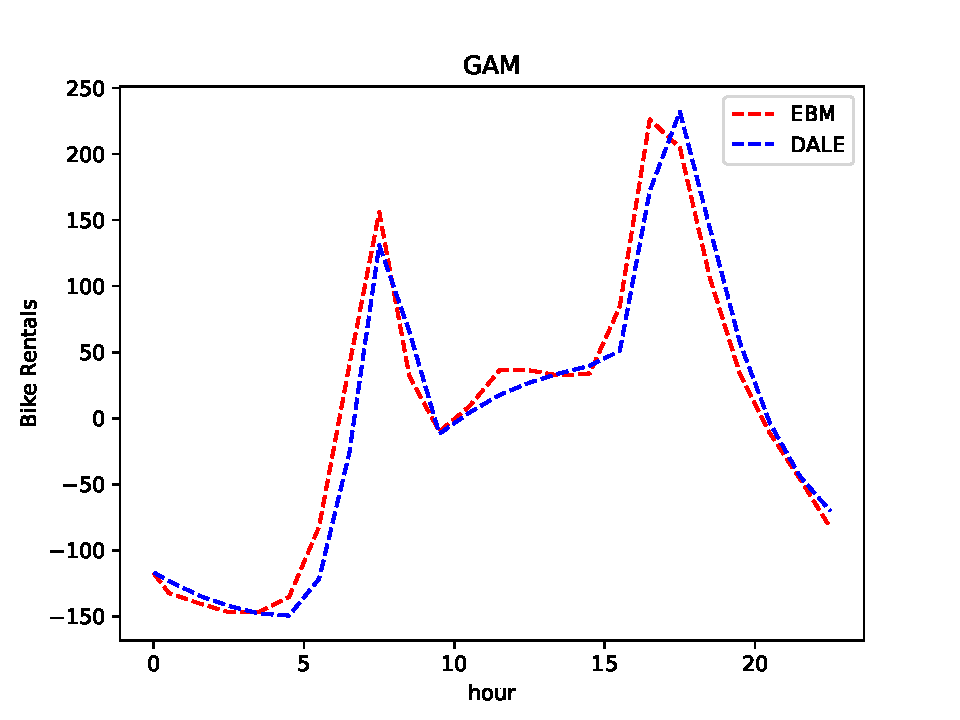
\includegraphics[width=\textwidth]{figures/bike_rentals_gam}
        \caption{\(f(X_{\mathtt{hour}})\)}
        \label{subfig:bike_rentals_gam}
    \end{subfigure}
    \begin{subfigure}{0.32\textwidth}
        \centering
        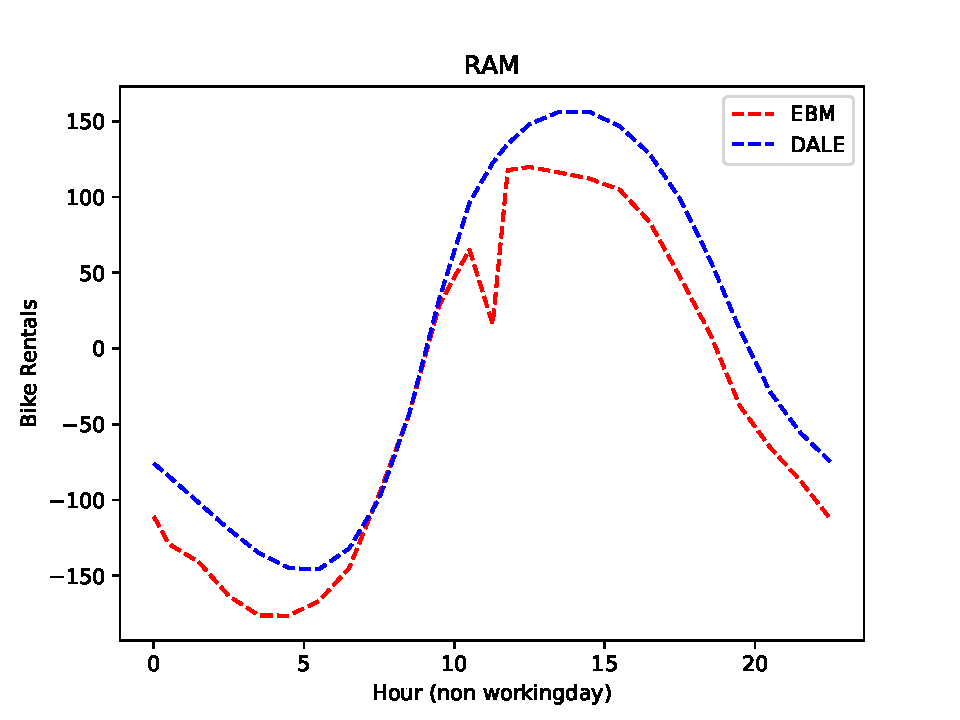
\includegraphics[width=\textwidth]{figures/bike_rentals_ram_1}
        \caption{\(f(X_{\mathtt{hour}}) \when{X_{\mathtt{workingday}} \neq 1}\)}
        \label{subfig:bike_rentals_regional_gam_1}
    \end{subfigure}
    \begin{subfigure}{0.32\textwidth}
        \centering
        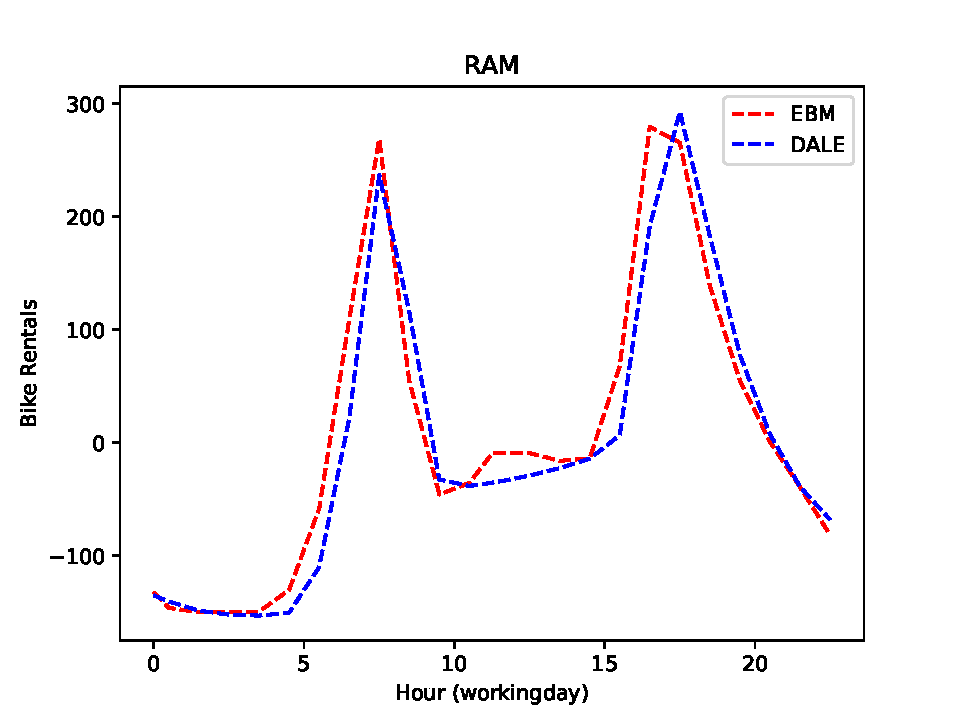
\includegraphics[width=\textwidth]{figures/bike_rentals_ram_2}
        \caption{\(f(X_{\mathtt{hour}}) \when{X_{\mathtt{workingday}} = 1}\)}
        \label{subfig:bike_rentals_regional_gam_2}
    \end{subfigure}
    \caption{Comparison of different models' predictions for bike rentals based on the hour of the day.
    Subfigure (a) depicts the generalized additive model (GAM),
        while subfigures (b) and (c) illustrate the RAM model's predictions for different day types: non-working days
        \(f(X_{\mathtt{hour}}) \when{X_{\mathtt{workingday}} \neq 1}\) and
        working days \(f(X_{\mathtt{hour}}) \when{X_{\mathtt{workingday}} = 1}\), respectively.
        The RAM model successfully captures the interaction between the hour of the day and the day type,
        leading to improved predictions and enhanced interpretability.}
    \label{fig:bike_sharing}
\end{figure}


\paragraph{California Housing Dataset}


The California Housing dataset consists of approximately $20,000$ of housing blocks situated in California.
Each housing block is described by eight numerical features, namely,
$X_{\mathtt{latitude}}$, $X_{\mathtt{longitude}}$, $X_{\mathtt{median\_age}}$, $X_{\mathtt{total\_rooms}}$, $X_{\mathtt{total\_bedrooms}}$, $X_{\mathtt{population}}$, $X_{\mathtt{households}}$, and $X_{\mathtt{median\_income}}$.
The target variable, $Y_{\mathtt{value}}$, is the median house value in dollars for each block.
The target value ranges in the interval \([15, 500] \cdot 10^3\), with a mean value of
\(\mu_Y \approx 201 \cdot 10^3 \) and a standard deviation of \(\sigma_Y \approx 110 \cdot 10^3\).

As a black-box model, we train for $45$ epochs a fully-connected Neural Network with 6 hidden layers,
using the Adam optimizer with a learning rate of $0.001$.
The model achieves a root mean square error (RMSE) of about \(40\)K dollars on the test set.
Subsequently, we perform subregion extraction by searching for splits up to a maximum depth of \(T=3\).
After the postprocessing step, we discover that several splits significantly reduce the level of interactions,
resulting in an expanded input space consisting of \(16\) features, as we show in table~\ref{tab:california_housing_subregions}.
Out of them, we randomly select and illustrate in Figure~\ref{fig:california_housing} the effect of the feature $X_{\mathtt{longitude}}$.
As we observe, for the house blocks located in the southern part of California ($X_{\mathtt{latitude}} \leq 34.9$),
the house value decreases in an almost linear fashion as we move eastward ($X_{\mathtt{longitude}}$ increases).
In contrast, for the house blocks located in the northern part of California ($X_{\mathtt{latitude}} > 34.9$),
the house value performs a rapid (non-linear) decrease as we move eastward ($X_{\mathtt{longitude}}$ increases).
We also observe that although the EBM fitted to each subregion captures the general trend,
it does not align perfectly with the regional effect.
As in the Bike-Sharing Example, the RMSE of the RAM model, i.e. \( 0.53 \cdot 110 \cdot 10^3 \approx 58.3 \cdot 10^3\) dollars on the test set,
is lower than the one of the GAM model, i.e.\( 0.6 \cdot 110 \cdot 10^3 \approx 66 \cdot 10^3\) dollars.
These results indicate that the RAM model provides superior predictions compared to the GAM model.
The same conclusion holds is when comparing the RAM$^2$ and the GAM$^2$ models.
\begin{table}[htbp]
  \centering
  \caption{California Housing: Subregions Detected by RAM}
  \label{tab:california_housing_subregions}
  \begin{tabular}{c|c|}
      Feature & Subregions \\
      \hline
      \multirow{2}{*}{$X_{\mathtt{longitude}}$} & $X_{\mathtt{longitude}} \when{X_{\mathtt{latitude}} \leq 34.9}$ \\
      & $X_{\mathtt{longitude}} \when{X_{\mathtt{latitude}} > 34.9}$ \\
      \hline
      \multirow{2}{*}{$X_{\mathtt{latitude}}$} & $X_{\mathtt{latitude}} \when{X_{\mathtt{longitude}} \leq -120.31}$ \\
      & $X_{\mathtt{latitude}} \when{X_{\mathtt{longitude}} > -120.31}$ \\
      \hline
      \multirow{2}{*}{$X_{\mathtt{total\_rooms}}$} & $X_{\mathtt{total\_rooms}} \when{X_{\mathtt{total\_bedrooms}} \leq 449.37}$ \\
        & $X_{\mathtt{total\_rooms}} \when{X_{\mathtt{total\_bedrooms}} > 449.37}$ \\
      \hline
      \multirow{4}{*}{$X_{\mathtt{total\_bedrooms}}$} & $X_{\mathtt{total\_bedrooms}} \when{X_{\mathtt{households}} \leq 411} \when{X_{\mathtt{total\_bedrooms}} \leq 647}$ \\
        & $X_{\mathtt{total\_bedrooms}} \when{X_{\mathtt{households}} \leq 411} \when{X_{\mathtt{total\_bedrooms}} > 647}$ \\
        & $X_{\mathtt{total\_bedrooms}} \when{X_{\mathtt{households}} > 411} \when{X_{\mathtt{total\_bedrooms}} \leq 647}$ \\
        & $X_{\mathtt{total\_bedrooms}} \when{X_{\mathtt{households}} > 411} \when{X_{\mathtt{total\_bedrooms}} > 647}$ \\
      \hline
      \multirow{2}{*}{$X_{\mathtt{population}}$} & $X_{\mathtt{population}} \when{X_{\mathtt{households}} \leq 411.5}$ \\
      & $X_{\mathtt{population}} \when{X_{\mathtt{households}} > 411.5}$ \\
      \hline
      \multirow{2}{*}{$X_{\mathtt{households}}$} & $X_{\mathtt{households}} \when{X_{\mathtt{total\_bedrooms}} \leq 630.57}$ \\
        & $X_{\mathtt{households}} \when{X_{\mathtt{total\_bedrooms}} > 630.57}$ \\
  \end{tabular}
\end{table}


\begin{figure}[htbp]
    \centering
    \begin{subfigure}{0.32\textwidth}
        \centering
        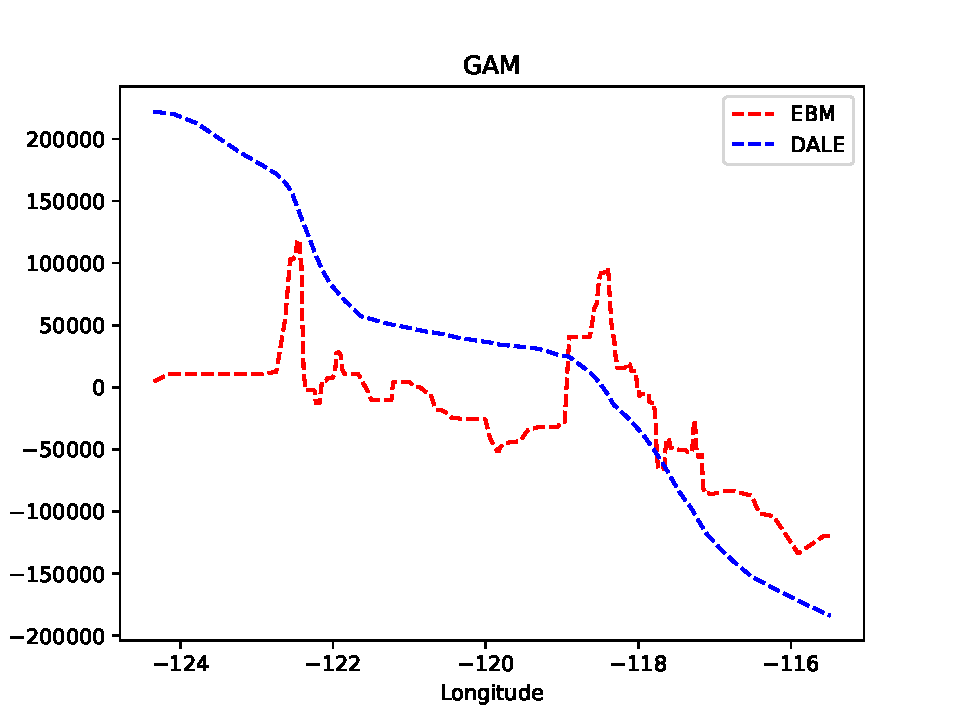
\includegraphics[width=\textwidth]{figures/california_gam}
        \caption{\(f(X_{\mathtt{longitude}})\)}
        \label{subfig:california_gam}
    \end{subfigure}
    \begin{subfigure}{0.32\textwidth}
        \centering
        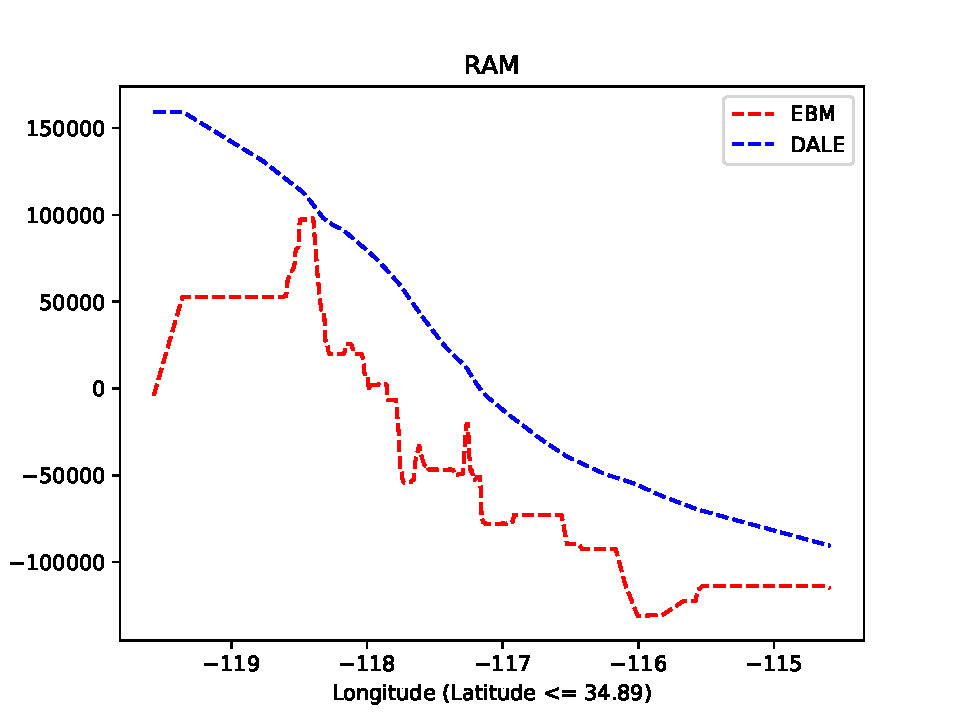
\includegraphics[width=\textwidth]{figures/california_ram_1}
        \caption{\(f(X_{\mathtt{longitude}}) \when{X_{\mathtt{latitude}} \leq 34.89}\)}
        \label{subfig:california_ram_1}
    \end{subfigure}
    \begin{subfigure}{0.32\textwidth}
        \centering
        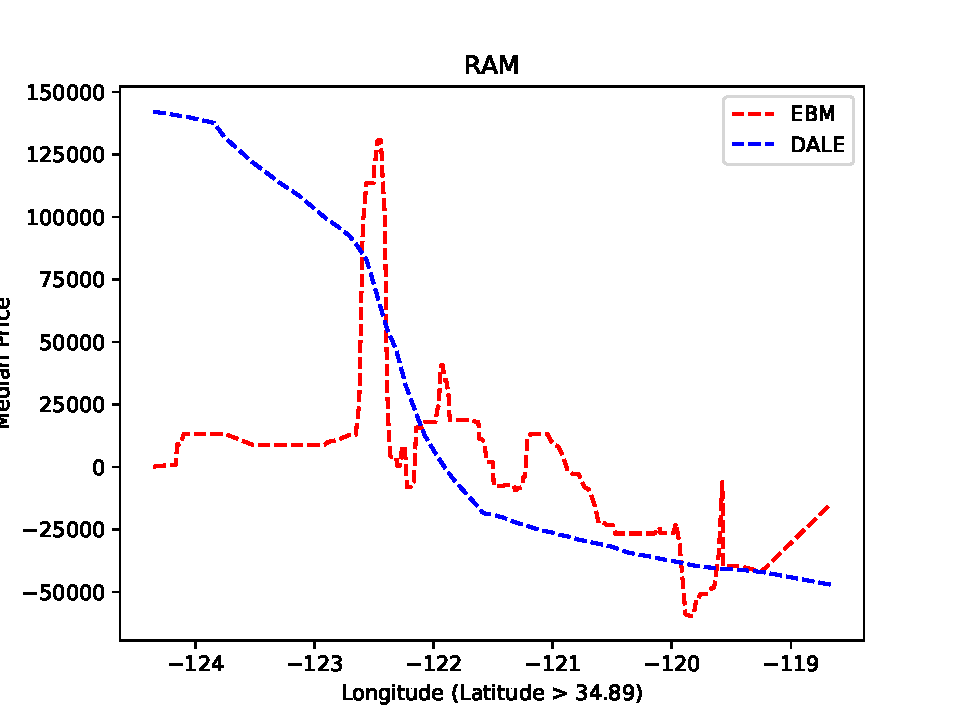
\includegraphics[width=\textwidth]{figures/california_ram_2}
        \caption{\(f(X_{\mathtt{longitude}}) \when{X_{\mathtt{latitude}} > 34.89}\)}
        \label{subfig:california_ram_2}
    \end{subfigure}
    \caption{Caption for the entire figure}
    \label{fig:california_housing}
\end{figure}

\section{Conclusion and Future Work}

In this paper we have introduced the Regional Additive Models (RAM) framework, a novel approach for learning accurate
x-by-design models from data.
RAMs operate by decomposing the data into subregions, where the relationship between the target variable and the
features exhibits an approximately additive nature.
Subsequently, Generalized Additive Models (GAMs) are fitted to each subregion and combined to create the final model.
Our experiments on two standard regression datasets have shown promising results, indicating that RAMs can provide more accurate predictions compared to GAMs while maintaining the same level of interpretability.

Nevertheless, there are still several unresolved questions that require attention and further experimentation.
Firstly, it is essential to systematically evaluate the performance of RAMs on a larger set of datasets to ensure that the observed improvements are not specific to particular datasets.
Secondly, we need to explore different approaches for each step of the RAM framework.
For the initial step, we should experiment with various black-box models.
Regarding the subregion detection step, we can explore alternative clustering algorithms.
Finally, in the last step, we should investigate different types of GAM models to fit within each subregion.

Another important area of investigation involves exploring the impact of second-order effects within the RAM framework.
While our experimenation demonstrated that even with the current subregion detection, RAM$^2$s outperform GAM$^2$s,
it may be the case, that for second-order models the optimal subregions are not necessarily those that maximize the additive effect of individual features,
but rather those that maximize the additive effect of feature pairs.

\section{Appendix}

\subsection{Regional DALE formulation}
\label{sec:regional_dale}

For this reason we define the bin-effect, the bin-deviation and the aggregated deviation on a subregion \(\mathcal{R}_{st}\) as:

\begin{equation}
    \label{eq:bin_effect_subregion}
    \hat{\mu}_{\mathcal{R}_{st}}(z_{k-1}, z_k) = \frac{1}{|\mathcal{S}_k \cap \mathcal{R}_{st}|} \sum_{i:\mathbf{x}^i \in \mathcal{S}_k \cap \mathcal{R}_{st} } \dfdx(\mathbf{x}^i)
\end{equation}

\begin{equation}
  \label{eq:bin_deviation_subregion}
  \hat{\sigma}_{\mathcal{R}_{st}}^2(z_{k-1}, z_k) = \frac{1}{|\mathcal{S}_k \cap \mathcal{R}_{st}| - 1}
\sum_{i:\mathbf{x}^i \in \mathcal{S}_k \cap \mathcal{R}_{st} } \left ( \dfdx(\mathbf{x}^i) -
    \hat{\mu}(z_{k-1}, z_k) \right )^2
\end{equation}

\begin{equation}
  \label{eq:SE}
  \mathcal{L}_{\mathcal{R}_{sk}} = \sum_{k=1}^K (z_k - z_{k-1})^2 \hat{\sigma}_{\mathcal{R}_{st}}^2(z_{k-1}, z_k)
\end{equation}

\subsection{Algorithmic Details of Subregion Detection}

\begin{algorithm}
\caption{SplitDataset}
\label{alg:split_dataset}
\SetAlgoLined
\SetKwInOut{Input}{Input}
\SetKwInOut{Output}{Output}
\Input{X\_list, J\_list, c, val, is\_cat}
\Output{X\_split, J\_split}
X\_split $\gets$ []\;
J\_split $\gets$ []\;
\For{i = 1 to len(X\_list)}{
    X= X\_list[i]\;
    J= J\_list[i]\;
    \uIf{is\_cat}{
        ind\_1 $\gets$ X[:, c] $=$ val\;
        ind\_2 $\gets$ X[:, c] $\neq$ val\;
    }
    \Else{
        ind\_1 $\gets$ X[:, c] $\leq$ val\;
        ind\_2 $\gets$ X[:, c] $>$ val\;
    }
    Append X[ind\_1], X[ind\_2] to X\_split\;
    Append J[ind\_1], J[ind\_2] to J\_split\;
}
\Return X\_split, J\_split
\end{algorithm}


\bibliography{report}






\end{document}
